\documentclass{standalone}
\usepackage{tikz}
\usepackage{amsmath}
\usetikzlibrary{arrows.meta, decorations.pathreplacing}

\begin{document}

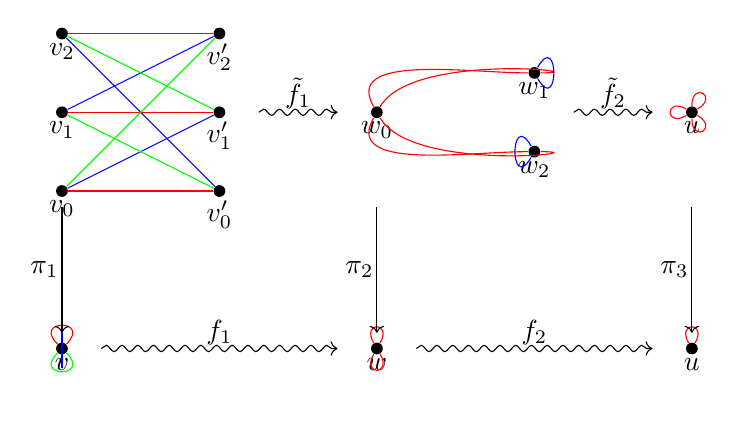
\begin{tikzpicture}[every node/.style={inner sep=1pt}]

% First graph (top left)
\node (v0) at (0,2) [circle,fill,inner sep=1.5pt,label=below:{$v_0$}] {};
\node (v1) at (0,3) [circle,fill,inner sep=1.5pt,label=below:{$v_1$}] {};
\node (v2) at (0,4) [circle,fill,inner sep=1.5pt,label=below:{$v_2$}] {};

\node (v0') at (2,2) [circle,fill,inner sep=1.5pt,label=below:{$v_0'$}] {};
\node (v1') at (2,3) [circle,fill,inner sep=1.5pt,label=below:{$v_1'$}] {};
\node (v2') at (2,4) [circle,fill,inner sep=1.5pt,label=below:{$v_2'$}] {};

\draw[red] (v0) -- (v0');
\draw[red] (v1) -- (v1');
\draw[red] (v2) -- (v2');

\draw[blue] (v0) -- (v1');
\draw[blue] (v1) -- (v2');
\draw[blue] (v2) -- (v0');

\draw[green] (v0) -- (v2');
\draw[green] (v1) -- (v0');
\draw[green] (v2) -- (v1');

% Second graph (top middle)
\node (w0) at (4,3) [circle,fill,inner sep=1.5pt,label=below:{$w_0$}] {};
\node (w1) at (6,3.5) [circle,fill,inner sep=1.5pt,label=below:{$w_1$}] {};
\node (w2) at (6,2.5) [circle,fill,inner sep=1.5pt,label=below:{$w_2$}] {};

\draw[red] (w0) to[out=120,in=180] (w1);
\draw[red] (w1) to[out=0,in=60] (w0);

\draw[red] (w0) to[out=240,in=180] (w2);
\draw[red] (w2) to[out=0,in=300] (w0);

\draw[blue] (w1) to[out=300,in=60,looseness=10] (w1);
\draw[blue] (w2) to[out=240,in=120,looseness=10] (w2);

% Third graph (top right)
\node (u) at (8,3) [circle,fill,inner sep=1.5pt,label=below:{$u$}] {};

\draw[red] (u) to[out=30,in=90,looseness=10] (u);
\draw[red] (u) to[out=150,in=210,looseness=10] (u);
\draw[red] (u) to[out=270,in=330,looseness=10] (u);

% First morphism (top)
\draw[->,decorate,decoration={snake,amplitude=.4mm,segment length=2mm}] (2.5,3) -- node[above] {$\tilde{f}_1$} (3.5,3);

% Second morphism (top)
\draw[->,decorate,decoration={snake,amplitude=.4mm,segment length=2mm}] (6.5,3) -- node[above] {$\tilde{f}_2$} (7.5,3);

% First base graph (bottom left)
\node (v) at (0,0) [circle,fill,inner sep=1.5pt,label=below:{$v$}] {};

\draw[red] (v) to[out=45,in=135,looseness=10] (v);
\draw[green] (v) to[out=180+45,in=180+135,looseness=10] (v);
\draw[blue] (v) to[out=90,in=180+90,looseness=10] (v);

% Second base graph (bottom middle)
\node (w) at (4,0) [circle,fill,inner sep=1.5pt,label=below:{$w$}] {};

\draw[red] (w) to[out=60,in=120,looseness=10] (w);
\draw[red] (w) to[out=180+60,in=180+120,looseness=10] (w);

% Third base graph (bottom right)
\node (u') at (8,0) [circle,fill,inner sep=1.5pt,label=below:{$u$}] {};

\draw[red] (u') to[out=60,in=120,looseness=10] (u');

% Projection arrows
\draw[->] (0,1.8) -- node[left] {$\pi_1$} (0,0.2);
\draw[->] (4,1.8) -- node[left] {$\pi_2$} (4,0.2);
\draw[->] (8,1.8) -- node[left] {$\pi_3$} (8,0.2);

% Lower morphisms
\draw[->,decorate,decoration={snake,amplitude=.4mm,segment length=2mm}] (0.5,0) -- node[above] {$f_1$} (3.5,0);
\draw[->,decorate,decoration={snake,amplitude=.4mm,segment length=2mm}] (4.5,0) -- node[above] {$f_2$} (7.5,0);

\end{tikzpicture}

\end{document}